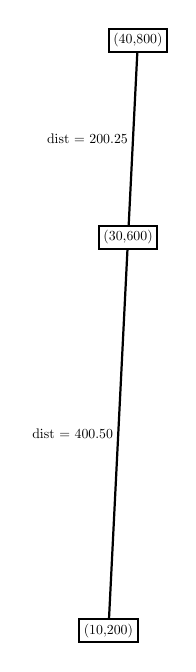
\begin{tikzpicture}[thick,scale=0.5, every node/.style={scale=0.5}]
    \begin{scope}
        \node[draw] (A) at (0.25,5) {(10,200)};
        \node[draw] (B) at (0.75,15) {(30,600)};
        \node[draw] (C) at (1.00,20) {(40,800)};
    \end{scope}

    \begin{scope}
        \draw (A) -- node[midway, left] {dist = 400.50} (B);
        \draw (B) -- node[midway, left] {dist = 200.25} (C);
    \end{scope}
\end{tikzpicture}